\makeatletter \def\input@path{{../../}} \makeatother
\documentclass[aspectratio=169]{beamer}
\usetheme{SimplePlus}

\usepackage{tikz}
\usepackage{amsmath}
\usepackage{amssymb}
\usepackage{bm}
\DeclareMathOperator{\grad}{\nabla}

\title[Traces and Poincar\'e]{Weak formulations and Galerkin schemes}
\author{Nicol\'as A. Barnafi}
\date{}

\begin{document}

\begin{frame}
    \titlepage
\end{frame}

\begin{frame}{Outline}
    \tableofcontents
\end{frame}

\section{Review and Boundary Conditions}

\begin{frame}{Density and Homogeneous Boundary Conditions}
    We can construct Sobolev spaces with boundary conditions using density.

    \vspace{0.3cm}
    For a pure homogeneous Dirichlet problem, $H^1_0(\Omega)$ is the closure of smooth functions with compact support:
    $$ H^1_0(\Omega) := \overline{C_0^\infty(\Omega)}^{\|\cdot\|_{1,\Omega}} $$

    This definition is rigorously equivalent to defining the space via the kernel of the trace operator: $H^1_0(\Omega) = \{v \in H^1(\Omega) : \gamma_0 v = 0 \text{ on } \partial\Omega\}$.

    \vspace{0.3cm}
    \textbf{Question:} How to consider Dirichlet conditions only on a portion $\Gamma_D \subset \partial\Omega$?
    $$ V_0 = \{ v \in H^1(\Omega) : \gamma_0 v = 0 \text{ on } \Gamma_D \} $$
\end{frame}

\begin{frame}{Partial Boundary Conditions via Density}
    \begin{columns}
        \begin{column}{0.65\textwidth}
            We define $V_0$ as the closure of smooth functions that vanish \textit{only} in a neighborhood of $\Gamma_D$.

            \vspace{0.2cm}
            Let $C^\infty_D(\bar{\Omega}) = \{ \phi \in C^\infty(\bar{\Omega}) : \text{supp}(\phi) \cap \Gamma_D = \emptyset \}$, then:
            $$ V_0 := \overline{C^\infty_D(\bar{\Omega})}^{\|\cdot\|_{1,\Omega}} $$

            \vspace{0.2cm}
            The construction is thus analogous.
        \end{column}
        \begin{column}{0.34\textwidth}
            \begin{center}
            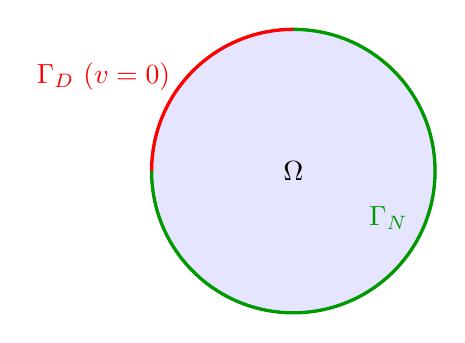
\begin{tikzpicture}[scale=1.2]
                % Domain
                \draw[thick, fill=blue!10] (0,0) to[out=90,in=180] (1.5,1.5) to[out=0,in=90] (3,0) to[out=270,in=0] (1.5,-1.5) to[out=180,in=270] (0,0);

                % Dirichlet Boundary
                \draw[very thick, red] (0,0) to[out=90,in=180] (1.5,1.5);
                \node[red, left] at (0.3, 1) {$\Gamma_D$ ($v=0$)};

                % Neumann Boundary
                \draw[very thick, green!60!black] (1.5,1.5) to[out=0,in=90] (3,0) to[out=270,in=0] (1.5,-1.5) to[out=180,in=270] (0,0);
                \node[green!60!black, right] at (2.2, -0.5) {$\Gamma_N$};

                \node at (1.5, 0) {$\Omega$};
            \end{tikzpicture}
            \end{center}
        \end{column}
    \end{columns}
\end{frame}

\section{Non-Homogeneous Boundary Conditions}

\begin{frame}{Problem Setup}
    Consider the Poisson problem where the Dirichlet condition is not zero:
    \begin{align*}
        -\Delta u &= f \quad \text{in } \Omega, \\
        \gamma_0 u &= g \quad \text{on } \Gamma_D.
    \end{align*}

    To formulate this weakly, we must separate the solution space from the test space.
    \begin{itemize}
        \item \textbf{Solution Space:} $V_g = \{ v \in H^1(\Omega) : \gamma_0 v = g \text{ on } \Gamma_D \}$
        \item \textbf{Test Space:} $V_0 = \{ v \in H^1(\Omega) : \gamma_0 v = 0 \text{ on } \Gamma_D \}$
    \end{itemize}

    \vspace{0.3cm}
    \textbf{The Weak Problem:} Find $u \in V_g$ such that
    $$ (\nabla u, \nabla v) = (f, v) \quad \forall v \in V_0 $$

    \vspace{0.2cm}
    \textit{The Analytical Issue:} $V_g$ is an affine space, not a vector space (it is not closed under addition). Consequently, we cannot directly apply the Lax-Milgram lemma.
\end{frame}

\begin{frame}{The Lifting Operator and Existence Analysis}
    To apply Lax-Milgram, we must shift the problem back to the vector space $V_0$. We do this via a \textbf{lifting function}.

    \vspace{0.2cm}
    As the trace operator is surjective onto $H^{1/2}(\Gamma_D)$, if $g \in H^{1/2}(\Gamma_D)$, there exists a lifting $u_g \in H^1(\Omega)$ such that $\gamma_0 u_g = g$.

    \vspace{0.2cm}
    \textbf{Decomposition:} We write the solution as $u = u_0 + u_g$, where $u_0 \in V_0$. Substituting this into the weak formulation yields:
    $$ (\nabla(u_0 + u_g), \nabla v) = (f, v) \quad \forall v \in V_0 $$

    \vspace{0.2cm}
    \textbf{The Modified Problem:} Find $u_0 \in V_0$ such that
    $$ (\nabla u_0, \nabla v) = (f, v) - (\nabla u_g, \nabla v) \quad \forall v \in V_0 $$

    \vspace{0.2cm}
    This is now a standard abstract problem $a(u_0, v) = \tilde{f}(v)$ defined entirely on the Hilbert space $V_0$. Lax-Milgram now applies for $u_0$ (and thus $u$).
\end{frame}

\section{From Weak to Strong Formulation}

\begin{frame}{The Fundamental Lemma of Calculus of Variations}
    To recover the strong PDE from the integral equation, we rely on localization.

    \begin{block}{Fundamental Lemma of Calculus of Variations}
        Let $\Omega \subset \mathbb{R}^d$ be bounded and $f \in L^1(\Omega)$. If
        $$ \int_\Omega f \phi \, dx = 0 \quad \forall \phi \in C_0^\infty(\Omega) $$
        then $f = 0$ almost everywhere.
    \end{block}
\end{frame}

\begin{frame}{Recovering the Strong Form: The Interior}
    Consider the weak mixed problem: Find $u \in V_0$ such that
    $$ (\nabla u, \nabla v) = (f, v) + \langle h, v \rangle_{\Gamma_N} \quad \forall v \in V_0 $$

    \textbf{Hypothesis:} Assume the weak solution possesses sufficient regularity, e.g., $u \in H^2(\Omega)$ or at least $\Delta u \in L^1(\Omega)$, so that classical differential operations hold almost everywhere.

    \vspace{0.2cm}
    \textbf{Step 1: Test in the interior.}
    Choose $v \in C_0^\infty(\Omega) \subset V_0$. The boundary term $\langle h, v \rangle_{\Gamma_N}$ vanishes. Integrating by parts yields:
    $$ (-\Delta u - f, v) = 0 \quad \forall v \in C_0^\infty(\Omega) $$

    By the Fundamental Lemma, we recover the PDE:
    $$ -\Delta u = f \quad \text{a.e. in } \Omega $$
\end{frame}

\begin{frame}{Recovering the Strong Form: The Boundary}
    \textbf{Step 2: Test on the boundary.}
    We know $-\Delta u = f$. Multiply by an arbitrary $v \in V_0$ and integrate by parts:
    $$ (\nabla u, \nabla v) - \langle \nabla u \cdot n, v \rangle_{\Gamma_N} = (f, v) $$

    Subtract this from the original weak formulation:
    $$ \langle \nabla u \cdot n - h, v \rangle_{\Gamma_N} = 0 \quad \forall v \in V_0 $$

    Since the trace of $V_0$ is dense in an appropriate boundary space on $\Gamma_N$, we conclude:
    $$ \nabla u \cdot n = h \quad \text{on } \Gamma_N $$
    We have successfully recovered the full boundary value problem.
\end{frame}

\section{Galerkin Schemes}

\begin{frame}{The (Discrete) Galerkin Problem}
    We restrict the continuous space $V$ to a finite-dimensional subspace $V_h \subset V$. We call this a \emph{conforming} approximation.

    \vspace{0.2cm}
    \textbf{The Discrete Problem:} Find $u_h \in V_h$ such that
    $$ a(u_h, v_h) = f(v_h) \quad \forall v_h \in V_h $$

    \vspace{0.2cm}
    \textbf{Galerkin Orthogonality:}
    Since $V_h \subset V$ (conformity), the true continuous solution $u \in V$ exactly satisfies $a(u, v_h) = f(v_h)$. Subtracting the discrete equation yields:
    $$ a(u - u_h, v_h) = 0 \quad \forall v_h \in V_h $$
    The error $e_h = u - u_h$ is orthogonal to the discrete test space with respect to $a(\cdot, \cdot)$.
\end{frame}

\begin{frame}{Well-Posedness of the Discrete Problem}
    Does the discrete problem have a unique solution? Yes, direct from conformity.

    \vspace{0.2cm}
    \begin{itemize}
        \item \textbf{Discrete Boundedness:}
        $$ |a(u_h, v_h)| \le C \|u_h\|_V \|v_h\|_V \quad \forall u_h, v_h \in V_h $$
        \item \textbf{Discrete Coercivity (Ellipticity):}
        $$ a(v_h, v_h) \ge \alpha \|v_h\|^2_V \quad \forall v_h \in V_h $$
    \end{itemize}

    \vspace{0.2cm}
    Since $V_h$ is a closed subspace (being finite-dimensional), Lax-Milgram guarantees a unique discrete solution $u_h \in V_h$ and uniform stability: $\|u_h\|_V \le \frac{1}{\alpha}\|f\|_{V'}$.
\end{frame}

\begin{frame}{C\'ea's Estimate}
    \begin{block}{Céa Estimate}
        For a conformal, consistent Galerkin scheme with an elliptic and continuous bilinear form, the error satisfies:
    $$ \|u - u_h\|_V \le \frac{C}{\alpha} \inf_{v_h \in V_h} \|u - v_h\|_V $$
    \end{block}

    \textbf{Proof:} Let $z_h \in V_h$ be an arbitrary discrete function.
    \begin{align*}
        \alpha \|u - u_h\|_V^2 &\le a(u - u_h, u - u_h) \quad \text{(Ellipticity)} \\
        &= a(u - u_h, u - z_h) + a(u - u_h, z_h - u_h) \\
        &= a(u - u_h, u - z_h) \quad \text{(Galerkin Orthogonality)} \\
        &\le C \|u - u_h\|_V \|u - z_h\|_V \quad \text{(Continuity)}
    \end{align*}
    Dividing by $\|u - u_h\|_V$ and taking the infimum over $z_h \in V_h$ yields the result. \qed
\end{frame}


\begin{frame}
    \titlepage
\end{frame}


\end{document}
